\section{Evaluation}

In this section, we evaluate \texttt{DepthFake} against three commercial liveness detection modules in the real world. 
We use the attack success rate (SR) as the metric to evaluate our attack, which is the ratio of the number of successful attacks against liveness detection modules over the total number of conducted attacks. 


\subsection{Experimental Setup}
\label{sec:experimental}

\begin{figure}[pt]
	\centerline{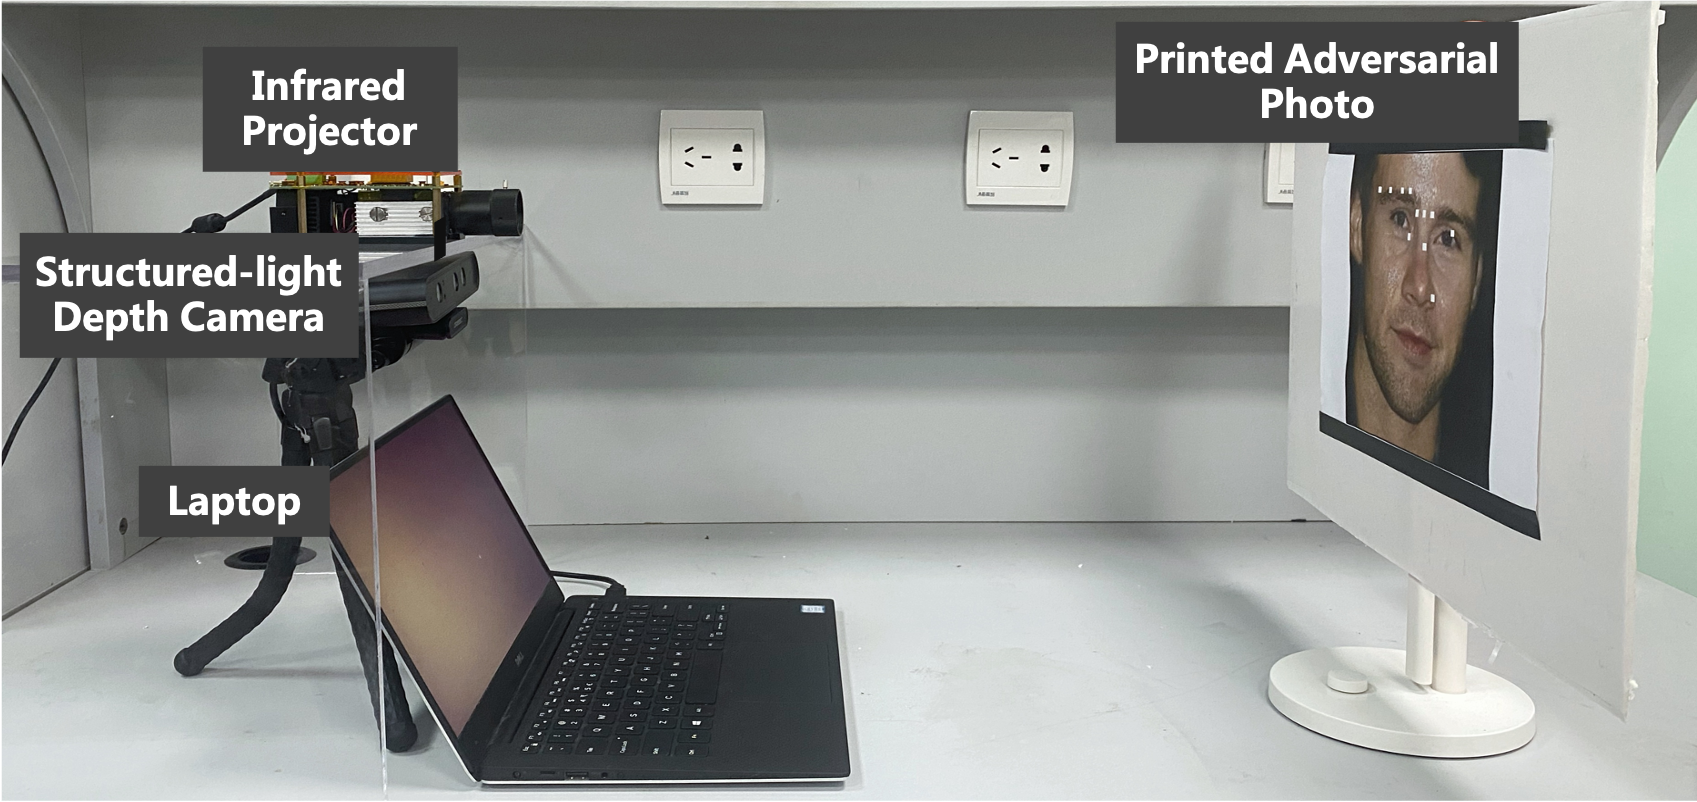
\includegraphics[width = 0.48\textwidth]{figures/setup.png}}
	\vspace{-0.1in}
	\caption{Experimental setup.   A infrared projector is used to project a structure-light scatter pattern onto an adversarial photo of a legitimate user  present in front of the target module to launch RGB-D attacks.}
	\vspace{-0.1in}
	\label{setup}
\end{figure}


\begin{table}[pt]
	\small 
	\caption{Default parameters during evaluation.}
	\vspace{-0.2in}
	\begin{center}
		\setlength{\tabcolsep}{1.5mm}{
			\renewcommand{\arraystretch}{1.2} 
			\begin{tabular}{c|c|c}
				\hline
				\textbf{Resolution} & \multicolumn{2}{c}{$640 \times 480$ pixels (480p)} \\
				\hline
				\multirow{2}{*}{\textbf{Light Condition}} & illumination intensity & $300~lx$ \\
				\cline{2-3}
				& color temperature & $6500~K$\\
				\hline
				\multirow{4}{*}{\textbf{Thresholds}} & Tencent Cloud & RGB: 0.4, Depth: 0.5 \\
				\cline{2-3}
				& Baidu Cloud & RGB: 0.8, Depth: 0.8 \\
				\cline{2-3}
				& 3DiVi & RGB: 0.9, Depth: 0.5 \\
				\hline
		\end{tabular}}
		\label{default_param}
	\end{center}
	\vspace{-0.15in}
\end{table}

\begin{table*}[t]
	\caption{Overall Performance of \texttt{DepthFake} attacks with four users against four different  liveness detection modules.}
	\vspace{-0.1in}
	\begin{center}
		\setlength{\tabcolsep}{6.5mm}{
			\renewcommand{\arraystretch}{1.2} 
			\begin{tabular}{c|c|c|c|c}
				\hline
				\multirow{2}{*}{\textbf{Datasets}} & \multirow{2}{*}{\textbf{Modalities}} & \multicolumn{3}{c}{\textbf{Target Systems}}                   \\
				\cline{3-5}
				& & Tencent Cloud & Baidu Cloud & 3DiVi \\
				\hline
				\hline
				\multirow{2}{*}{300W-3D} & Depth
				& \textit{74.1\%} (THR:0.4) &  \textit{68.0\%} (THR:0.8) & \textit{95.2\%} (THR:0.5) \\
				\cline{2-5}
				& RGB-D
				& \textit{49.0\%} (THR:0.4, 0.5) & \textit{45.0\%} (THR:0.8, 0.8) & \textit{71.2\%} (THR:0.9, 0.5) \\
				\hline
				\multirow{2}{*}{Texas-3DFR} & Depth
				& \textit{73.2\%} (THR:0.4) &  \textit{70.2\%} (THR:0.8) & \textit{94.3\%} (THR:0.5) \\
				\cline{2-5}
				& RGB-D
				& \textit{45.1\%} (THR:0.4, 0.5) & \textit{38.0\%} (THR:0.8, 0.8) & \textit{56.2\%} (THR:0.9, 0.5) \\
				\hline
				\multirow{2}{*}{Volunteers} & Depth
				& \textit{71.3\%} (THR:0.5) &  \textit{64.5\%} (THR:0.8) & \textit{98.5\%} (THR:0.5) \\
				\cline{2-5}
				& RGB-D
				& \textit{71.3\%} (THR:0.4, 0.5) & \textit{63.8\%} (THR:0.8, 0.8) & \textit{72.3\%} (THR:0.9, 0.5) \\
				\hline
		\end{tabular}}
		\label{overall}
	\end{center}
	\vspace{-0.1in}
\end{table*}

\textbf{Target systems.} 
We use a commercial 3D camera Orbbec Astra Pro~\cite{da2020comparison} equipped with an RGB camera and a structured light depth camera as the hardware part of our target systems, as shown in Fig.~\ref{setup}. 
%The scatter projector of the structured light depth camera can project a fixed infrared structured light scatter pattern. 
We use three commercial face authentication SDKs/APIs as the software part of the target systems and try to spoof their liveness detection modules, including (1) Tencent Cloud~\cite{tencent}, (2) Baidu Cloud~\cite{baidu}, and (3) 3DiVi Face~\cite{3divi}. We deploy these SDKs/APIs on a DELL XPS 13 laptop and acquire the liveness confidence scores by calling interfaces.

\textbf{Attack Devices.} We use an infrared projector DLP4500SL02 Evaluation Module~\cite{chong2017intraoperative} as the attack device to project the modulated structured light scatter pattern, which has a resolution of $1280 \times 800$ pixels, and a projecting image size of $270~mm \times 168~mm$.
In addition, we use a printed adversarial photo of a legitimate user placed in front of the camera to spoof the RGB-based liveness detection, as shown in Fig.~\ref{setup}.

\textbf{Default Attack Setting.} During the experiments, we put the infrared projector above the target 3D camera with a distance of $20~mm$ and fix the distance between the projector and the adversarial photo as $500~mm$.
All the adversarial photos are printed with a  size of $400~mm \times 300~mm$.
Other default settings including the camera resolution, the light condition, and the thresholds of target systems are shown in Tab.~\ref{default_param}.

%The default background illumination intensity is $400~lx$ and the color temperature is $6500~K$. The default camera resolution is 480p, i.e., $640\times480$ pixels. The default thresholds of the target systems are as follows: (1) Tencent Cloud (RGB: 0.4, RGB-D: 0.4 for RGB and 0.5 for Depth), (2) Baidu Cloud (RGB: 0.8, RGB-D: 0.8 for RGB and 0.8 for Depth), (3) ArcFace (RGB: 0.5), (4) Huawei Cloud (RGB: 0.5).

\textbf{Datasets.} We evaluate our attacks on two datasets 300W-3D~\cite{zhu2016face} and Texas-3DFR~\cite{gupta2010anthropometric, gupta2010texas}. 
The 300W-3D dataset contains more than 3800 facial images with different genders, ages, races, illumination conditions, pose, occlusion, and face sizes. 
The Texas-3DFR dataset contains 1149 pairs of facial images from 105 adults of different genders, ages, and races.
For each dataset, we select 20 images with different genders, ages, and races to launch \texttt{DepthFake}.


\textbf{Volunteers.} We recruit five volunteers including three males and two females to evaluate the effectiveness of \texttt{DepthFake} attacks in the real world. The approval of the Institutional ReviewBoard (IRB) of our evaluation is in the application.

%\begin{figure*}[h!]
%	\centering
%	\subfigure[Attack Success Rates on various light conditions.]{
%		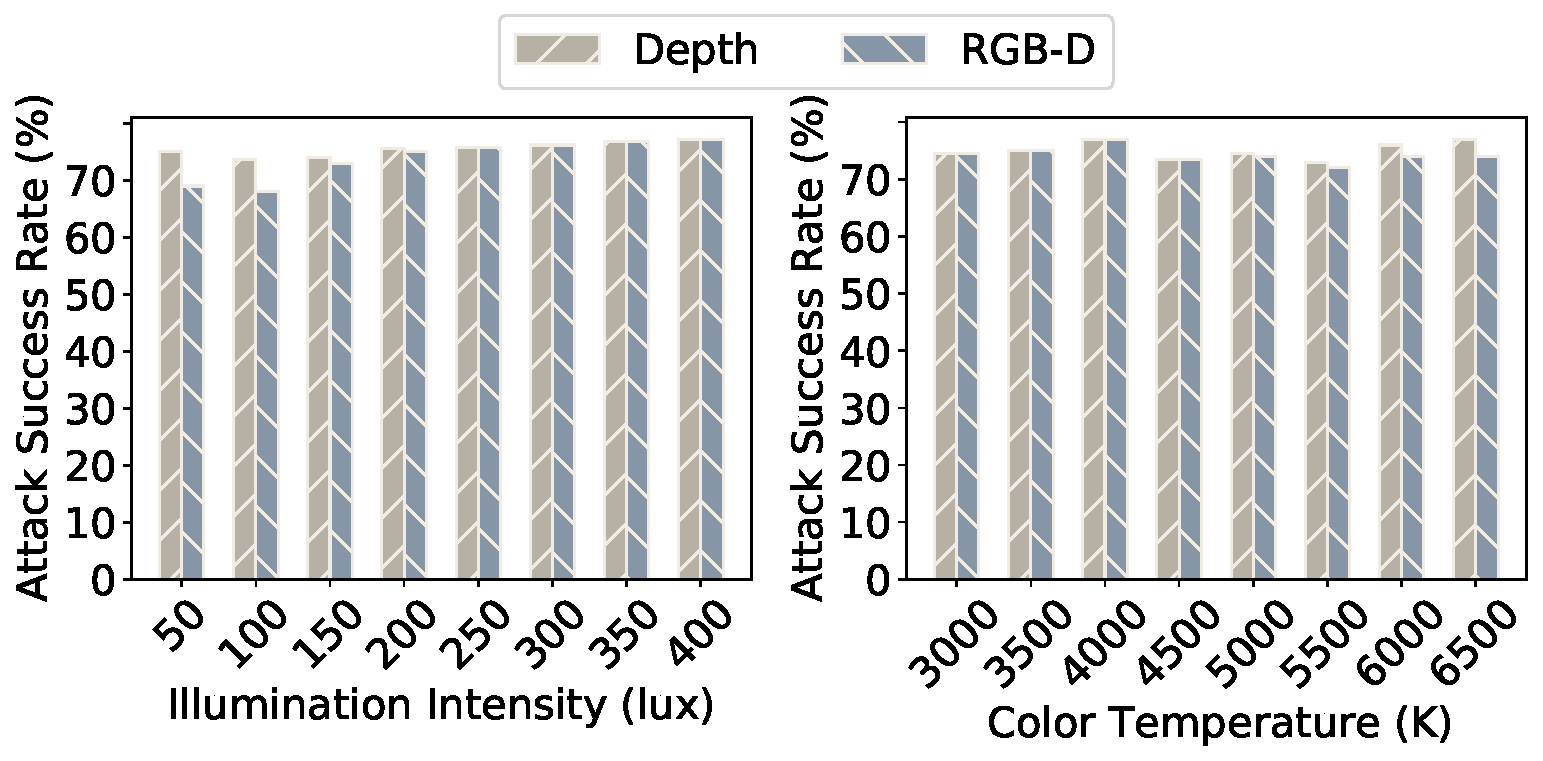
\includegraphics[width=0.48\textwidth]{figures/light_condition.pdf}
%	}
%	\subfigure[Confidence Scores on various light conditions.]{
%		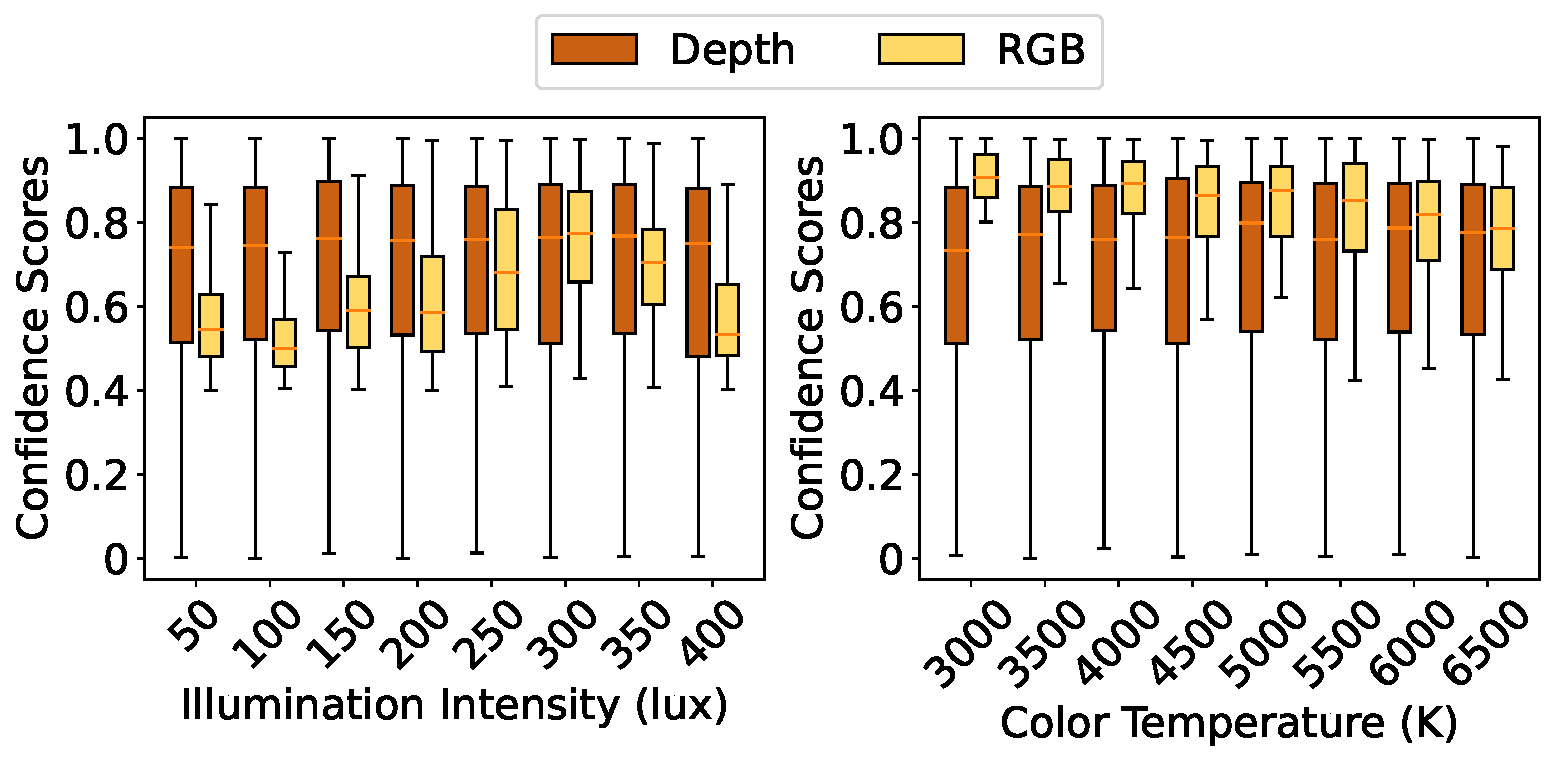
\includegraphics[width=0.48\textwidth]{figures/light_condition_scores.pdf}
%	}
%	\vspace{-0.1in}
%	\caption{Impact of \texttt{DepthFake} under various light conditions}
%	\label{light_condition}
%	\vspace{-0.1in}
%\end{figure*}

\begin{figure}[pt]
	\centerline{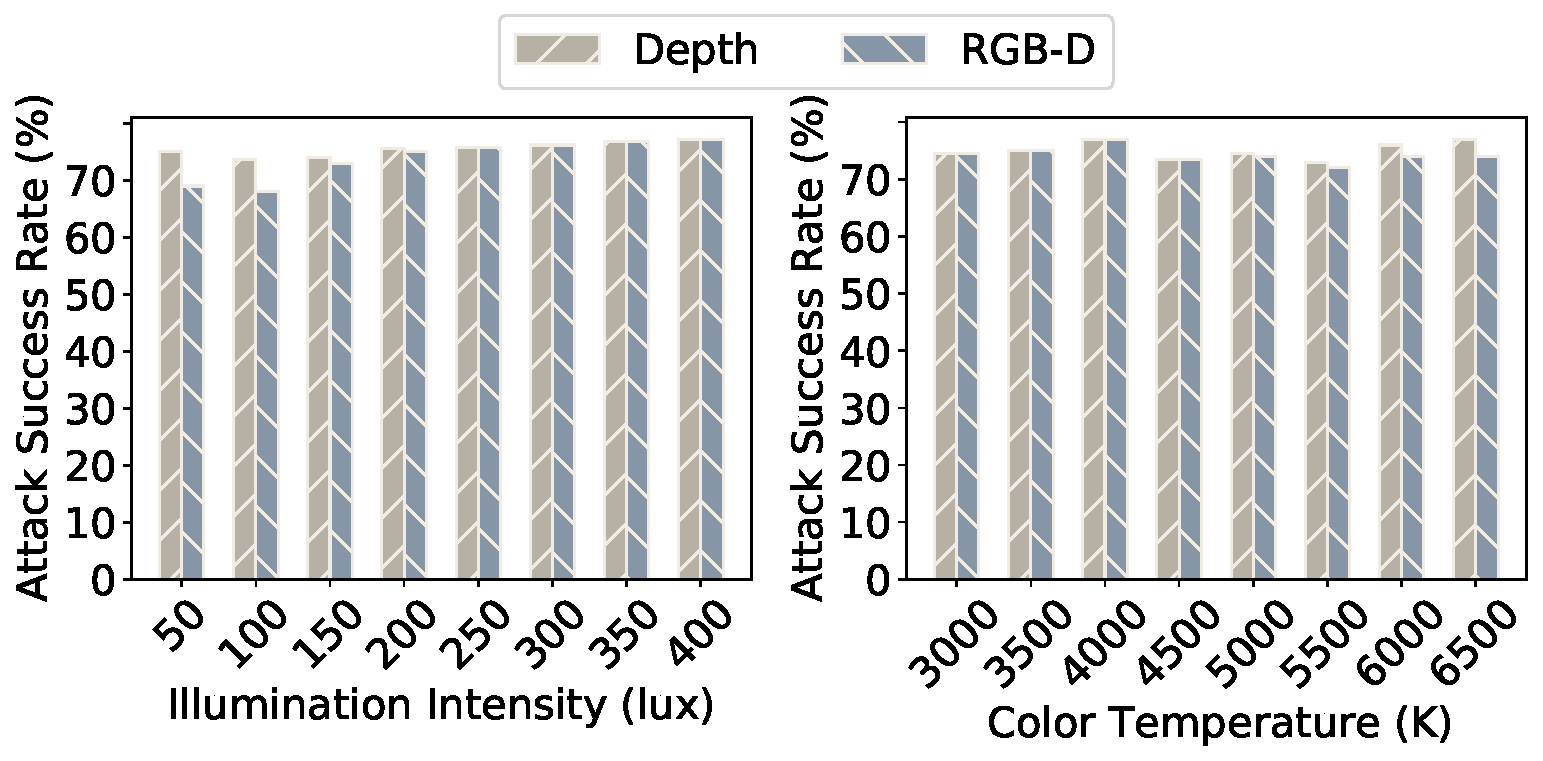
\includegraphics[width = 0.48\textwidth]{figures/light_condition.pdf}}
	\vspace{-0.15in}
	\caption{Impact of \texttt{DepthFake} attacks under various light conditions.}
	\label{light_condition}
	\vspace{-0.1in}
\end{figure}


\subsection{Overall Performance}
We first evaluate the overall performance of the Depth and RGB-D attacks on different people against three commercial liveness detection modules, i.e., Tencent Cloud, Baidu Cloud, and 3DiVi, under the default setting. 
The results shown in Tab.~\ref{overall} demonstrate that the Depth attacks can achieve an overall attack success rate of $72.8\%$ against Tencent Cloud, $67.6\%$ against Baidu Cloud, and $96\%$ against 3DiVi. The RGB-D attacks can achieve an overall attack success rate of $55.1\%$ against Tencent Cloud, $48.9\%$ against Baidu Cloud, and $66.6\%$ against 3DiVi.  Among two datasets and volunteers, the attack performance of the RGB-D attacks on volunteers is better than that on the 300W-3D dataset or the Texas-3DFR dataset. The reason is that some images in these  datasets are of poor quality, leading to the reduced performance of the RGB-D attacks. 
Among the three tested systems, 3DiVi is the most vulnerable while Baidu Cloud is the least. The reason is that Baidu Cloud uses higher default thresholds for both the RGB and Depth liveness detection. 
Another finding is that RGB-D based liveness detection is more difficult to attack compared with the Depth-based one. The reason is that the RGB-D attacks require the alignment of RGB and depth images but the projection distortion caused by the alignment process can lead to the reduction in attack performance.

Overall, our attack can achieve an attack success rate  over $63.8\%$ for the Depth attacks and $38\%$ for the RGB-D attacks against different people and systems.

%Overall, all of our attacks can achieve over $38\%$ attack success rate for both different datasets and target systems, which means that we can successfully attack the liveness detection every 3 times on average. However, commercial face authentication systems generally provide 5 to 10 opportunities for users to validate, so that, our attack can easily attack the liveness detection module in commercial face authentication systems.


%Among the three tested systems, Tencent Cloud is most vulnerable while Baidu Cloud is least vulnerable. The reason is that Baidu Cloud uses a higher default threshold during the liveness detection. 
%Another finding is Depth-based liveness detection is more difficult to attack compared with the RGB-D ones, resulting in the attack performance decrease in RGB-D attacks. Therefore, 3D liveness detection does better secure the process of face authentication compared with those 2D methods. 

%RGB modality can reach over than $90\%$ within the target system with a low default threshold, and get $61\%$ in a target system with high default threshold, which is proved that the RGB livness detection algorithms based on machine learning or deep learning is suffering from the threat of adversarial examples. The Depth modality performs the worst in our attack, but the attack success rate is still over than $44\%$. One reason is that the algorithm for generating depth information from structured-light scatter patterns requires precise scatter positions, so that a small offset may cause deviations in depth generation. Although our attack can extract an essentially complete structured-light scatter pattern, it still be disturbed by noise during the projection and imaging process, which may lead to deviations in depth generation. 
%
%Overall, all of our attacks can achieve over $32\%$ attack success rate for both different people and target systems (shown in in Appendix Tab.~\ref{overall}), which means that we can successfully attack the liveness detection in every 3 times on average. However, commercial face authentication systems generally provide 5 to 10 opportunities for users to validate, so that, our attack can easily attack the livenss detection module in commercial face authentication systems.



\subsection{Impact of Light Condition}

Then, we evaluate the light condition that may influence the attack effectiveness of \texttt{DepthFake}, including the illumination intensity and the color temperature. During the experiments, we use Tencent Cloud SDK with default thresholds as our target system and one volunteer as the victim.  
To avoid the mutual interference between the light intensity and color temperature, we keep the color temperature to $6500~K$ when evaluating the impact of the illumination intensity, and keep the illumination intensity to $300~lx$ when evaluating the impact of the color temperature.

\textbf{Illumination Intensity.} To investigate the impact of the illumination intensity on our attack, we set the background illumination intensity from $50~lx$ to $400~lx$ to conduct experiments.
From the results shown in Fig.~\ref{light_condition} (left), we find that both the Depth attacks and the RGB-D attacks can achieve average attack success rates of over $70\%$.
When the illumination intensity drops to $100~lx$, the attack success rate of the RGB-D attacks shows a slight decrease.
The reason is that the camera suffers from more noises when capturing images at a low illumination intensity. Another finding is that the attack performance at $50~lx$ is better than that of $100~lx$. It is because the camera will compensate for the exposure when the illumination intensity is too low.
At the same time, the attack success rate of the Depth attacks remains $\geq$$70\%$ across different illumination intensities. The reason is that the structured light depth camera uses an infrared scatter pattern to generate depth information, which is not subject to the interference from visible lights.


\textbf{Color Temperature.} Similar to illumination intensity, our attack may be affected by the color temperature. To investigate its impact, we conduct experiments by setting the background color temperature from $3000~lx$ to $6500~lx$.
The results are shown in Fig.~\ref{light_condition} (right). From the results, we find that the attack performance of both the Depth and RGB-D  attacks are unaffected as the color temperature changes, with attack success rates higher than $70\%$.
%The results of RGB attacks are shown in Fig.~\ref{color_temp} (a). From the results, we find that the attack success rates under the default threshold (0.4) reach $99\%$ in different color temperatures. With higher thresholds of 0.6 and 0.8, the attack success rate decreases as the color temperature rise, indicating that the RGB adversarial photo performs better at low color temperatures.%The attack success rate in $3000~K$ color temperature can reach over $90\%$ under a threshold of 0.8, 
%The results of RGB-D attacks are shown in Fig.~\ref{color_temp} (b). Similar to the illumination intensity, the color temperature of visible lights does not impact the performance of depth replay attacks. The RGB-D attacks can achieve an average attack success rate of $44.1\%$ with a depth threshold of 0.5.

Therefore, for the impact of light conditions, we find that (1)  light conditions have impacts on the RGB-D attacks but hardly affect the Depth attacks because they are based on infrared lights, and (2) \texttt{DepthFake} attacks can achieve an attack success rate of over $70\%$ under most light conditions.

\begin{figure}[pt]
	\centerline{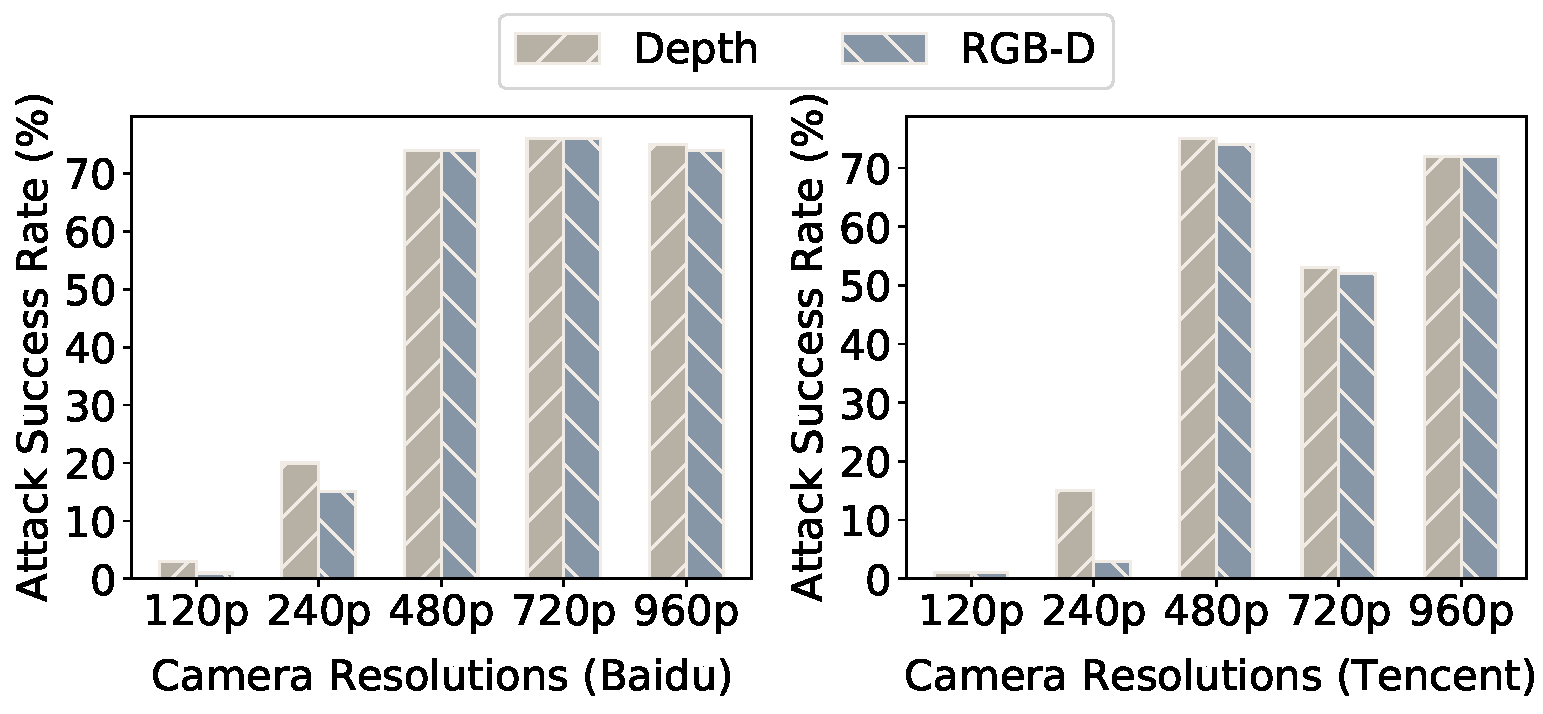
\includegraphics[width = 0.48\textwidth]{figures/camera_resolution.pdf}}
	\vspace{-0.15in}
	\caption{The attack effectiveness of \texttt{DepthFake} attacks under various camera resolutions.}
	\label{camera_resolution}
	\vspace{-0.15in}
\end{figure}


\begin{figure*}[pt]
	\centerline{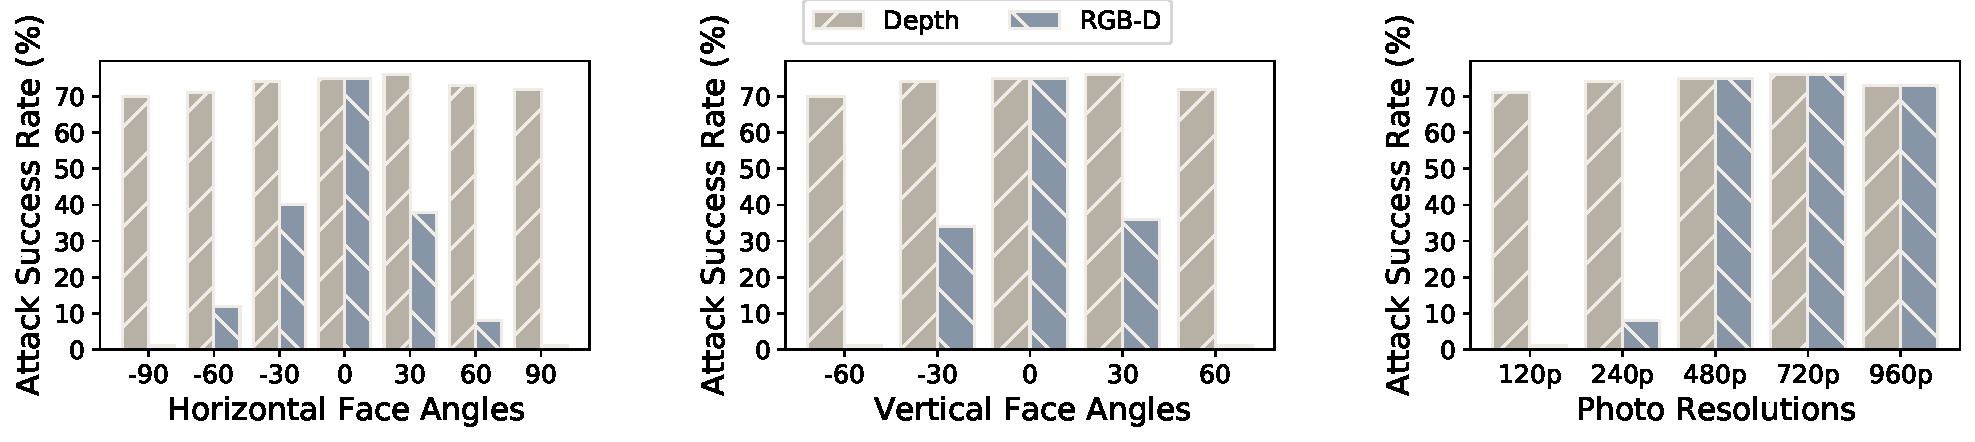
\includegraphics[width = \textwidth]{figures/photo_quality.pdf}}
	\vspace{-0.15in}
	\caption{The attack effectiveness of \texttt{DepthFake} attacks under various photo qualities. }
	\label{photo_quality}
	\vspace{-0.15in}
\end{figure*}

\subsection{Impact of Camera Resolution} 
Commercial face authentication systems may use cameras of various resolutions to capture images, which may influence the performance of our attack. To study its impact, we conduct experiments by using cameras of different resolutions including 120p, 240p, 480p, 720p, and 960p. During the experiments, we employ Tencent Cloud and Baidu Cloud as our victim systems, where the former uses the entire image for detection while the latter only uses the face region. 

From the results shown in Fig.~\ref{camera_resolution},  we find that the attack success rates of both the Depth and RGB-D attacks against two victim systems decline  when the camera resolution drops to 240p. The reasons are: 
(1) For Depth images, the lower camera resolution may cause the forged depth image to lose the 3D geometry structure of the human face.
(2) For RGB adversarial photos, the reduction in camera resolutions can weaken the attack effectiveness of the adversarial perturbations. 
%For instance, if the resolution is reduced from 480p to 120p, the face area will be compressed to a quarter of its original size. Thus, the face geometry can be lost and the $5\times5$ pixel adversarial units may also be compressed to one pixel or less, making them easily interfered by noises during imaging.

In addition, we find that with a camera resolution of 720p, the attack success rate against Tencent Cloud is lower than that of Baidu Cloud. The reason is that 720p images use a aspect ratio of $16:9$, while 480p images (default resolution) use $4:3$. Since Tencent Cloud uses the full image  for detection, the change in the aspect ratio will make the image different from the printed adversarial example, leading to a decrease in the effectiveness of the RGB attack. On the contrary, Baidu Cloud uses the face area for detection, which is not affected by the aspect ratio since the face area ratio is fixed.

Therefore, \texttt{DepthFake} attacks work better with cameras with high resolutions. However, with today's trend of using high-resolution cameras for surveillance, we assume \texttt{DepthFake} attacks still has its threat in the real world.

%\begin{figure}[pt]
%	\centering
%	\subfigure[Impact of camera resolutions (Baidu)]{
%		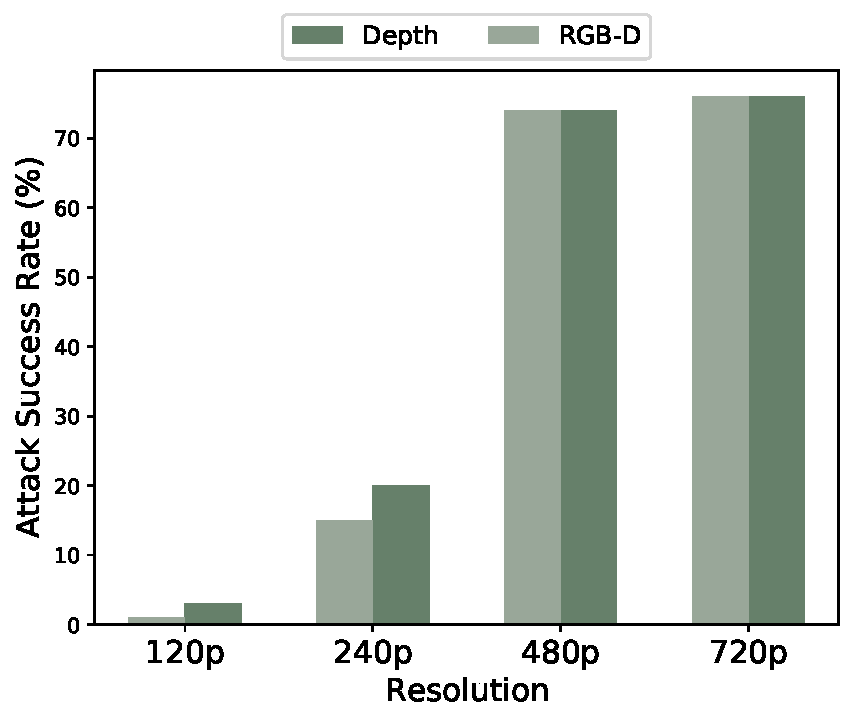
\includegraphics[width=0.22\textwidth]{figures/resolution_rgb_baidu.pdf} 
%	}
%	\hfill
%	\subfigure[Impact of camera resolutions (Tencent)]{
%		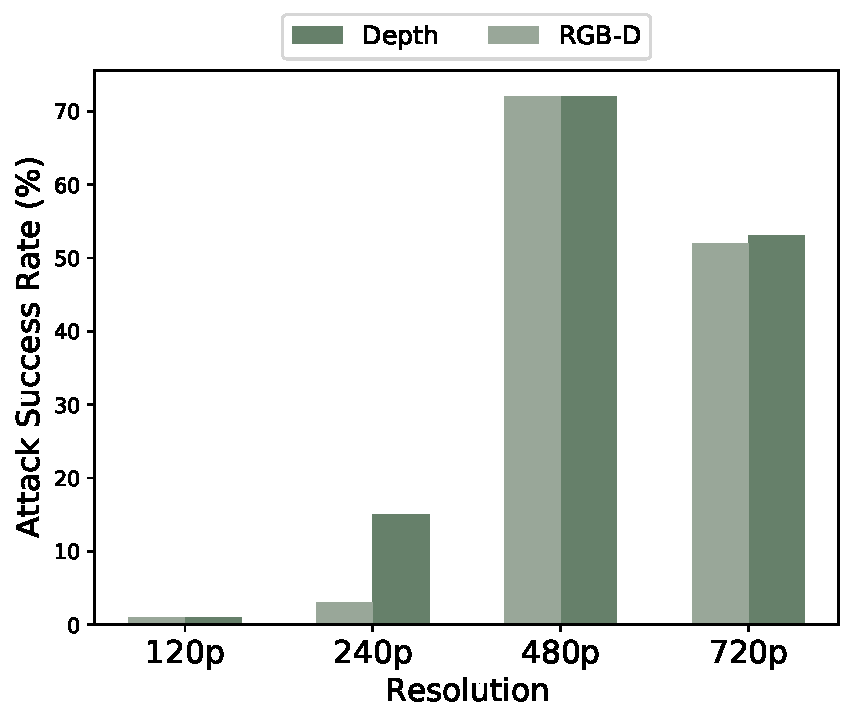
\includegraphics[width=0.22\textwidth]{figures/resolution_rgb_tencent.pdf} 
%	}
%	\vspace{-0.1in}
%	\caption{The attack effectiveness of \texttt{DepthFake} under various camera resolutions.}
%	\label{resolution}
%	\vspace{-0.1in}
%\end{figure}

\subsection{Impact of Photo Quality}
The public photos we obtained from victims' social medias are usually with different face angles and resolutions. In this subsection, we evaluate the attack effectiveness of our attacks under photos with different face angles and resolutions.

%\begin{figure}[pt]
%	\centering
%	\subfigure[Impact of face angle in horizontal]{
%		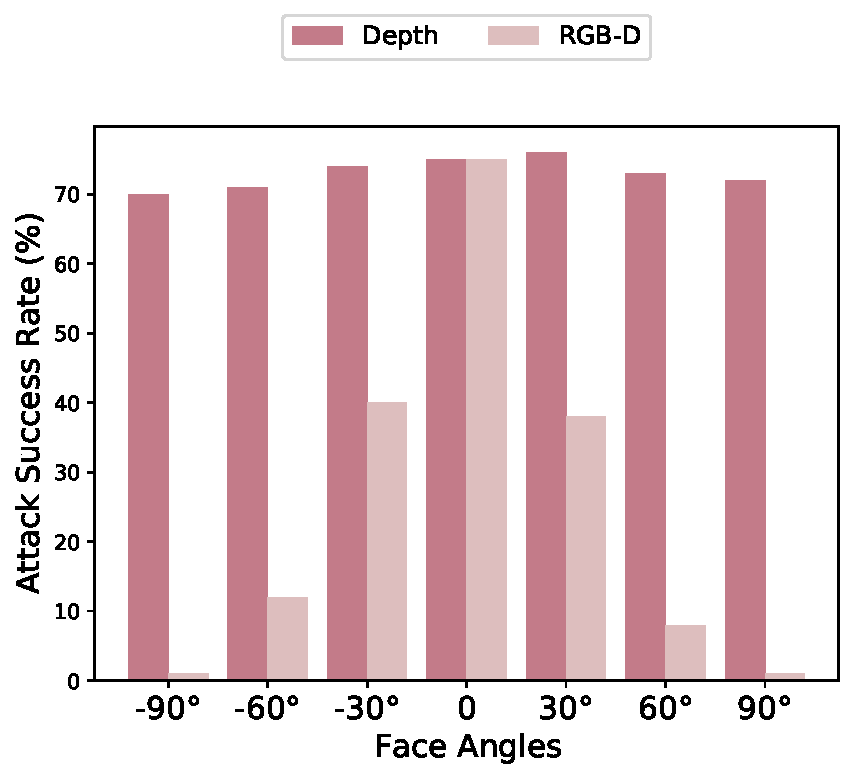
\includegraphics[width=0.22\textwidth]{figures/face_angle_horizontal.pdf} 
%	}
%	\hfill
%	\subfigure[Impact of face angle in vertical]{
%		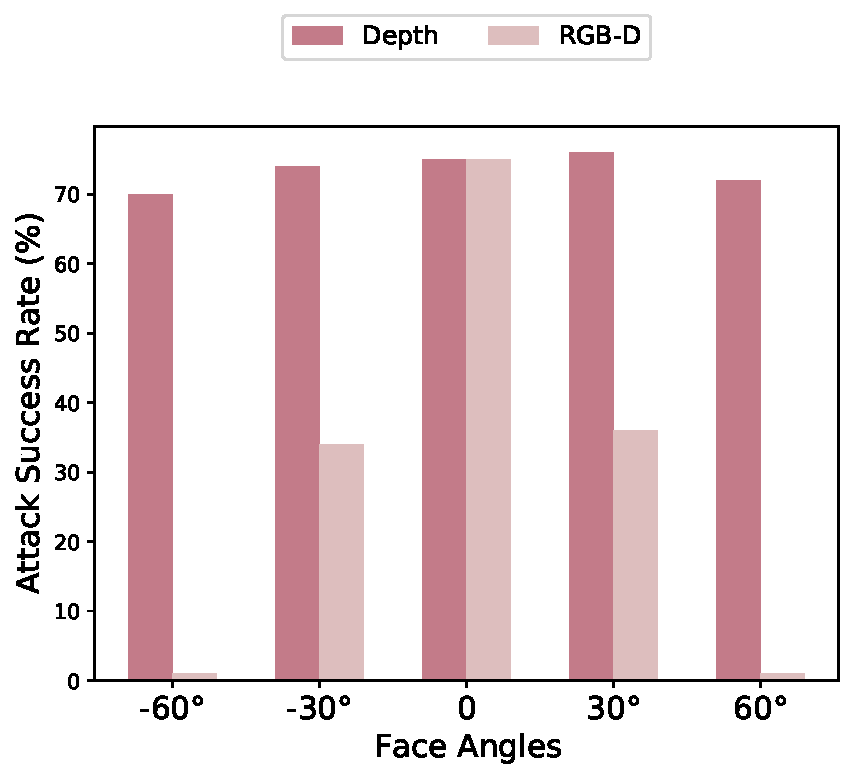
\includegraphics[width=0.22\textwidth]{figures/face_angle_vertical.pdf} 
%	}
%	\vspace{-0.1in}
%	\caption{The attack effectiveness of \texttt{DepthFake} under various face angles.}
%	\label{face_angle}
%	\vspace{-0.1in}
%\end{figure}

\textbf{Face Angles.}
To investigate the impact of face angles, we use images with different face angles in both horizontal (from $-90^\circ$ to $90^\circ$) and vertical  ($-60^\circ$ to $60^\circ$) directions to conduct experiments. 
%The face angles in the horizontal direction are from $-90^\circ$ to $90^\circ$, and the face angles in the vertical direction are from $-60^\circ$ to $60^\circ$.

The results are shown in Fig.~\ref{photo_quality}. For the depth attack, we find that the attack success rate can achieve over $70\%$ at any face angle. 
For the RGB-D attack, the attack success rate is susceptible to the face angle.
For both the horizontal and vertical directions, the attack success rate can achieve over $35\%$ when the face angle is between $-30^\circ$  to $30^\circ$. However, when the face angle is larger than $60^\circ$, the performance of the RGB-D attack decreases.
The reason is that when the face angle increases, the facial information contain in the photo decreases, increasing the difficulty of the RGB adversarial attack and thus the RGB-D attack.



%\begin{figure}[pt]
%	\centering
%	\subfigure[Impact of Photo Resolution]{
%		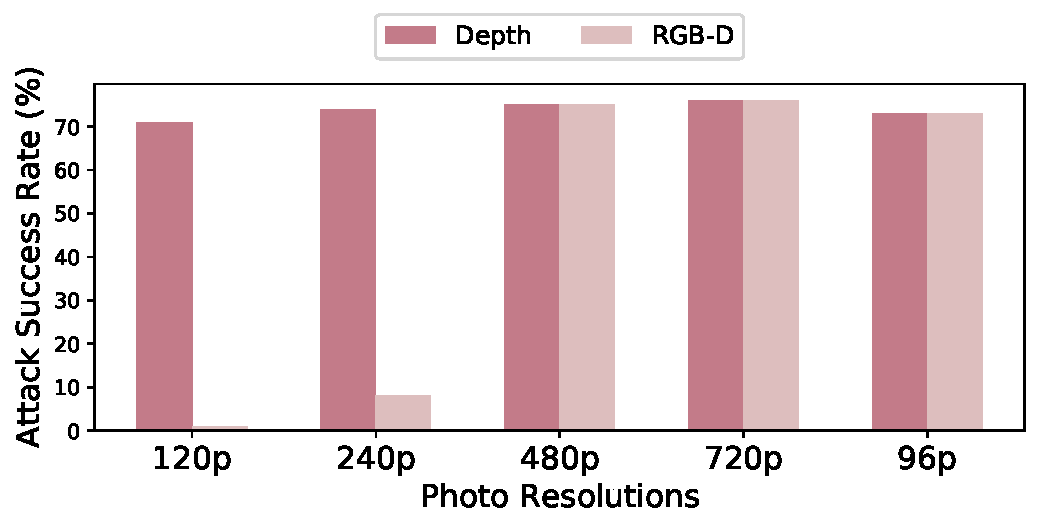
\includegraphics[width=0.45\textwidth]{figures/photo_resolution.pdf} 

%	}
%	\vspace{-0.1in}
%	\caption{The attack effectiveness of \texttt{DepthFake} under various photo resolution.}
%	\label{photo_resolution}
%	\vspace{-0.1in}
%\end{figure}

\textbf{Photo Resolutions.}
To evaluate the impact of photo resolutions, we use photos with different resolutions, i.e., 960p, 720p, 480p, 240p, and 120p, to conduct experiments. From the results shown in Fig.~\ref{photo_quality}, we find that both Depth and  RGB-D attacks can achieve attack success rates over $70\%$ on photos with resolutions larger than 480p. 
However, when the image resolution drops to 240p, the performance of the RGB-D attack decreases.
The reason is that the RGB-based liveness detection model can detect the blurred images and output them as 'non-living'. 
For the Depth attack, it is not affected by low image resolutions since: (1) In the depth estimation phase, our training dataset contains various resolution photos, which makes the depth estimation model robust to low-resolution photos. (2) In the depth forgery phase, the scatter pattern we modulate is not related to the resolution of the original RGB photo.

Therefore, \texttt{DepthFake} attacks work better with  public photos with face angles $\leq 30^\circ$ and image resolutions $\geq$480p.


\subsection{Impact of Relative Position}

\texttt{DepthFake} attacks use an external infrared projector to project the forged scatter pattern to an adversarial photo to launch RGB-D attacks. As a result, the relative position between the camera and the projector may distort the scatter pattern and thus influence the depth generation. In this subsection, we evaluate the attack effectiveness of Depth and RGB-D attacks under different camera-projector distances.

\textbf{Horizontal Distance.} We put the projector $2~cm$ above the camera and change their horizontal distance from  $0~cm$ to $12~cm$ to evaluate the impact of horizontal distances. From the results shown in Fig.~\ref{realted_position} (top), we find that the attack success rates for both the Depth and RGB-D attacks drop as the horizontal distance increases. 
With a horizontal distance of $4~cm$, both the Depth  and RGB-D attacks can achieve attack success rates of about $70\%$. However, when the relative horizontal distance is larger than $6~cm$, the attack success rate is reduced to $30\%$. The reason is that the depth generation highly depends on the location of the scatter pattern. The severe perspective distortion caused by the long horizontal distance will shift the projected scatter, resulting in the attack performance decrease. 

\textbf{Vertical Distance.} To evaluate the impact of vertical distances, we set the horizontal distance between the projector and camera to be  $0~cm$ and change its vertical distance from $2~cm$ to $8~cm$. The minimal vertical distance is set to $2~cm$ instead of $0~cm$ since the 3D camera has a shell of $2~cm$.The results shown in Fig.~\ref{realted_position} (bottom) demonstrate that the performance of the Depth attack and the RGB-D attack declines as the vertical distance increases. Nevertheless, both the Depth and RGB-D attacks can achieve  attack success rates over  $60\%$ when the vertical distance is less than $5~cm$. 
% It indicates that the depth generation of the structured-light camera is more sensitive to vertical distortion. 

Therefore, \texttt{DepthFake} attacks can tolerate a horizontal or vertical distance within $5~cm$ between the projector and the camera.



\begin{figure}[pt]
	\centerline{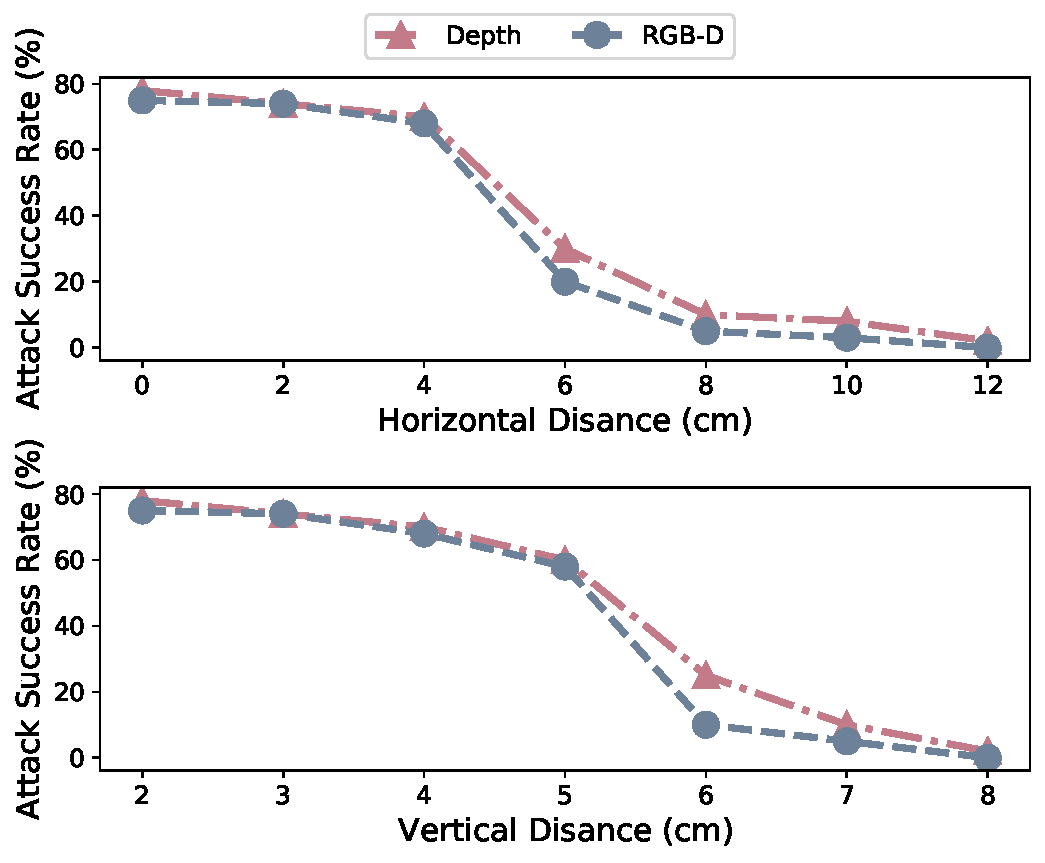
\includegraphics[width = 0.48\textwidth]{figures/related_position.pdf}}
	\vspace{-0.15in}
	\caption{Impact of relative positions between the camera and projector on \texttt{DepthFake} attacks. }
	\label{realted_position}
	\vspace{-0.1in}
\end{figure}


%\begin{figure}[!t]
%	\centering
%	\subfigure[Impact of hrizontal distances.]{
%		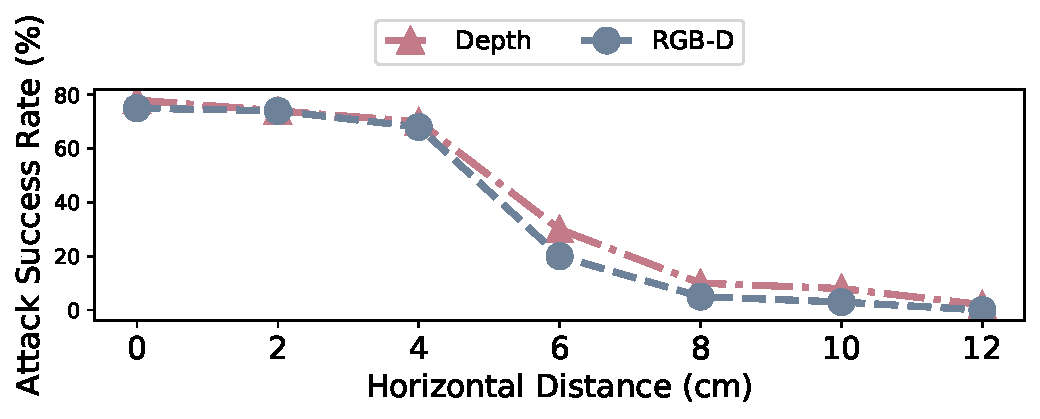
\includegraphics[width=0.45\textwidth]{figures/position_horizontal.pdf} 
%	}
%	\subfigure[Impact of vertical distances.]{
%		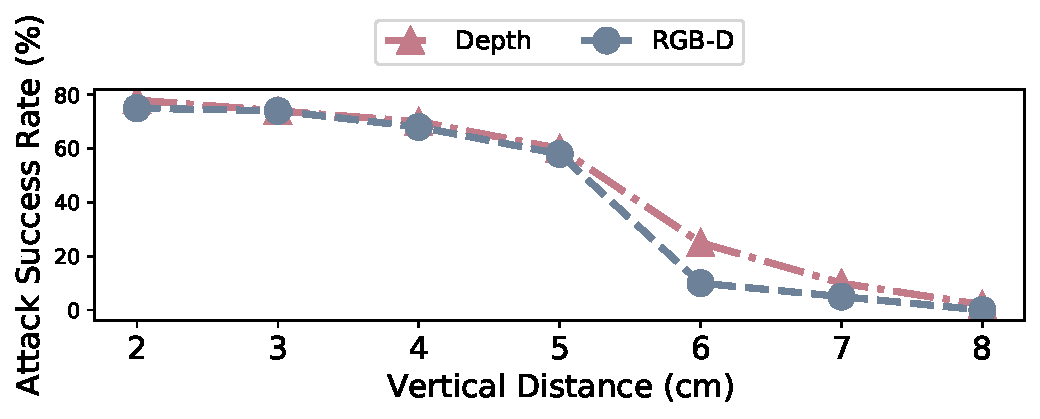
\includegraphics[width=0.45\textwidth]{figures/position_vertical.pdf} 
%	}
%	\vspace{-0.15in}
%	\caption{Impact of relative positions of the camera and projector on \texttt{DepthFake} attacks. }
%	\vspace{-0.2in}
%	\label{Position}
%\end{figure}

\subsection{End-to-End Face Authentication}

The \texttt{DepthFake} attack targets at the 3D liveness detection module in the commercial face authentication systems, based on the hypothesis that if we bypass the 3D liveness detection,  the face authentication system can be spoofed with a single photo.
To verify it,  we conduct experiments against end-to-end face authentication systems. Specifically, we evaluate the attack effectiveness of \texttt{DepthFake} attacks against each module in the standard workflow of face authentication systems, including face detection, liveness detection, and face comparison. 

We conduct an experiment with five users against three face authentication systems with their default thresholds.
For the results shown in Tab.~\ref{end2end}, we find that \texttt{DepthFake} attacks can pass every step of the face authentication system and successfully spoof the entire system. Moreover, we find that once the liveness detection step is bypassed, the following face comparison step can be $100\%$ spoofed. The reason is that \texttt{DepthFake} attacks do not make any changes to the face presentation features of the legitimate user. Furthermore, most commercial face authentication systems only rely on RGB images for face comparisons. The adversarial perturbation units we generate are small and sparse, and thus do not affect the face comparison step.


\begin{table}[pt]
	\caption{Attack Effectiveness of \texttt{DepthFake} attacks on  end-to-end face authentication systems.}
	\vspace{-0.2in}
	\begin{center}
		\setlength{\tabcolsep}{3.5mm}{
			\renewcommand{\arraystretch}{1.2} 
			\begin{tabular}{c|c|c|c}
				\hline
				\multirow{3}{*}{\textbf{Target Systems}} & \multicolumn{3}{c}{\textbf{Workflow of Face Authentication System}}  \\
				\cline{2-4}
				& Face       & Liveness   & Face      \\
				& Detection & Detection    & Comparison     \\
				\hline
				\hline
				Tencent Cloud & 100\% & 71.3\% & 100\%   \\
				\hline
				Baidu Cloud  & 100\% & 63.8\% & 100\%  \\
				\hline
				3DiVi      & 100\%& 92.3\% & 100\%  \\
				\hline
		\end{tabular}}
		\label{end2end}
	\end{center}
	\vspace{-0.1in}
\end{table}


%\subsection{Case Study: Entrance Guard System}
%To showcase the performance of our work on commercial devices in the real world, we validate our attack on an entrance guard device called \textit{Dumu CM Mini}. The \textit{Dumu CM Mini} is deployed with the Baidu Cloud SDK and uses RGB-IR modalities for liveness detection. Thus, we can transfer the RGB adversarial example from the attack against Baidu Cloud SDK. We put the printed adversarial example for RGB modality attack and use projector to relay the infrared image for IR modality attack. 
%
%The authentication result is shown in Figure.~\ref{commercial device}. Before we launch our attack, the \textit{Dumu CM Mini} rejects the access request and raises the access exception. Then, we replace the adversarial photo and turn on the infrared projector for RGB-IR replay attack. As shown in Figure.~\ref{commercial device} (b), our attack successful pass the access request to the \textit{Dumu CM Mini}. It is demonstrated that our attacks can transfer to commercial devices and our attack can be a serious threat to real-world Entrance Guard Systems.
%
%\begin{figure}[htbp]
%	\centering
%	\subfigure[Before attack]{
%		\includegraphics[width=0.225\textwidth]{figures/dumu_1.png} 
%	}
%	\subfigure[After attack]{
%		\includegraphics[width=0.225\textwidth]{figures/dumu_2.png} 
%	}
%	\caption{Performance on commercial device. }
%	\label{commercial device}
%\end{figure}